\documentclass{beamer}
\usepackage[utf8]{inputenc}

\usetheme{Madrid}
\usecolortheme{default}
\usepackage{amsmath,amssymb,amsfonts,amsthm}
\usepackage{txfonts}
\usepackage{tkz-euclide}
\usepackage{listings}
\usepackage{adjustbox}
\usepackage{array}
\usepackage{tabularx}
\usepackage{lmodern}
\usepackage{circuitikz}
\usepackage{tikz}
\usepackage{graphicx}

\setbeamertemplate{page number in head/foot}[totalframenumber]

\usepackage{tcolorbox}
\tcbuselibrary{minted,breakable,xparse,skins}

% Background color for code boxes
\definecolor{bg}{gray}{0.95}
\DeclareTCBListing{mintedbox}{O{}m!O{}}{%
  breakable=true,
  listing engine=minted,
  listing only,
  minted language=#2,
  minted style=default,
  minted options={%
    linenos,
    gobble=0,
    breaklines=true,
    fontsize=\small,
    numbersep=8pt,
    #1},
  boxsep=0pt,
  left skip=0pt,
  right skip=0pt,
  left=25pt,
  right=0pt,
  top=3pt,
  bottom=3pt,
  arc=5pt,
  leftrule=0pt,
  rightrule=0pt,
  bottomrule=2pt,
  toprule=2pt,
  colback=bg,
  colframe=orange!70,
  enhanced,
  overlay={%
    \begin{tcbclipinterior}
    \fill[orange!20!white] (frame.south west) rectangle ([xshift=20pt]frame.north west);
    \end{tcbclipinterior}},
}

% Set listings settings for C language
\lstset{
    language=C,
    basicstyle=\ttfamily\small,
    keywordstyle=\color{blue},
    stringstyle=\color{orange},
    commentstyle=\color{green!60!black},
    numbers=left,
    numberstyle=\tiny\color{gray},
    breaklines=true,
    showstringspaces=false,
}

% Define command for column vector and bold vector letter
\newcommand{\myvec}[1]{\ensuremath{\begin{pmatrix}#1\end{pmatrix}}}
\renewcommand{\vec}[1]{\boldsymbol{#1}} % bold vectors

% Meta Info
\title{4.2.20}
\date{September, 2025}
\author{Mahesh Chollangi - EE25BTECH11017}

\begin{document}

\frame{\titlepage}

\section*{Question}
\begin{frame}{Question}
Find the direction and normal vector for the line 
    x + 2y = 6
\end{frame}

\begin{frame}{Theoretical Solution}
Define the vectors:
\begin{equation}
  \vec{x} = \myvec{x \\ y}, \quad
    \vec{n} = \myvec{1 \\ 2}, \quad
    c = 6
    \label{eq:vecs_def}
\end{equation}
The line equation can be expressed as the dot product:
\begin{equation}
    \vec{n}^\top \vec{x} = c
    \label{eq:line_vec_eq}
\end{equation}
where \(\vec{n}\) is the normal vector.
\end{frame}

\begin{frame}{Direction Vector}
The direction vector \(\vec{m}\) is perpendicular to the normal vector \(\vec{n}\). It can be taken as:
\begin{equation}
    \vec{m} = \myvec{2 \\ -1}
    \label{eq:direction_vec}
\end{equation}

This follows since, if the direction vector is given by
\begin{equation}
    \vec{m} = \myvec{1 \\ m}
    \label{eq:direction_repr}
\end{equation}
then the normal vector is
\begin{equation}
    \vec{n} = \myvec{-m \\ 1}.
    \label{eq:normal_repr}
\end{equation}
\end{frame}

\begin{frame}{Verification of Orthogonality}
Verify that \(\vec{n}\) and \(\vec{m}\) are orthogonal:
\begin{equation}
    \vec{n}^\top \vec{m} = 0
    \label{eq:orthogonality_cond}
\end{equation}

Calculate:
\begin{equation}
    \myvec{1 & 2} \myvec{2 \\ -1} = 0
    \label{eq:orthogonality_calc}
\end{equation}
which confirms orthogonality.
\end{frame}

\begin{frame}{Final Answer}
\begin{enumerate}
    \item Normal vector: \(\vec{n} = \myvec{1 \\ 2}\)
    \item Direction vector: \(\vec{m} = \myvec{2 \\ -1}\)
\end{enumerate}
\end{frame}

\begin{frame}[fragile]{C Code}
\begin{lstlisting}
// Normal vector components
double normal[2] = {1, 2};

// Direction vector components (perpendicular to normal)
double direction[2] = {2, -1};

// Function to get normal vector pointer
double* get_normal() {
    return normal;
}

// Function to get direction vector pointer
double* get_direction() {
    return direction;
}
\end{lstlisting}
\end{frame}

\begin{frame}[fragile]{Python Code}
\begin{lstlisting}
import numpy as np
import matplotlib.pyplot as plt

# Line equation: x + 2y = 6
# Solve for y: y = (6 - x)/2

x = np.linspace(0, 7, 100)
y = (6 - x)/2

# Normal vector
n = np.array([1, 2])
# Direction vector (perpendicular to normal)
d = np.array([2, -1])

# Plot line
plt.plot(x, y, label='Line: x + 2y = 6')
\end{lstlisting}
\end{frame}

\begin{frame}[fragile]{Python Code (continued)}
\begin{lstlisting}
# Plot normal vector starting from point (3, 1.5) on the line (3 + 2*1.5 = 6)
origin = np.array([3, 1.5])

plt.quiver(*origin, *n, color='red', scale=3, label='Normal vector n = (1, 2)')
plt.quiver(*origin, *d, color='green', scale=3, label='Direction vector d = (2, -1)')

plt.xlim(0, 7)
plt.ylim(0, 5)
plt.xlabel('x')
plt.ylabel('y')
plt.title('Line with normal and direction vectors')
plt.grid(True)
plt.legend()
plt.show()
\end{lstlisting}
\end{frame}

\begin{frame}{Plot}
\centering
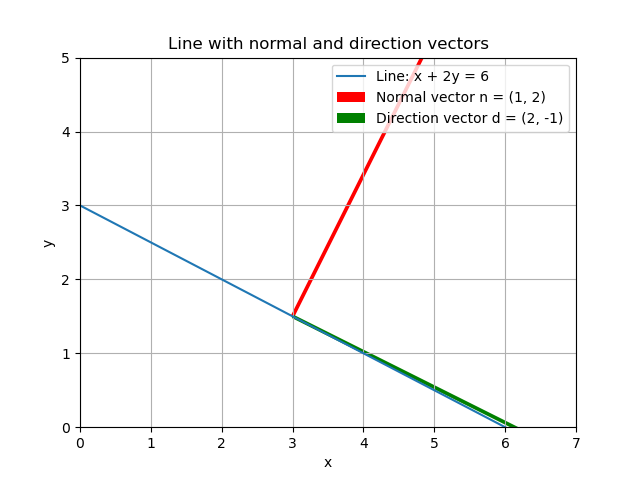
\includegraphics[width=0.85\textwidth,height=0.6\textheight,keepaspectratio]{Figs/Figure_4.png}
\end{frame}
\end{document}
